\documentclass[eng, 12pt, twoside, openany]{mgr}

\usepackage{hyperref}
\usepackage{polski}
\usepackage[utf8]{inputenc}
\usepackage{caption}
\usepackage{graphicx}
\usepackage{pdflscape}
\usepackage{pgfplots}
\pgfplotsset{compat=1.7}

\usepackage{floatrow}
\usepackage[section]{minted}
\usepackage{csquotes}
\setminted[cpp]{breaklines,linenos,fontsize=\footnotesize,tabsize=4,baselinestretch=1}
\newenvironment{kod}{  \captionsetup{type=listing} \vspace{1em} }{}

% Spis listingów
\renewcommand{\listoflistingscaption}{Spis listingów}
\renewcommand{\listoflistings}{
%   \cleardoublepage
  \phantomsection
  \addcontentsline{toc}{section}{\listoflistingscaption}
  \listof{listing}{\listoflistingscaption}
}

\author{Marcin Bober}
\title{Projekt systemu sensorycznego bazującego na protokole MQTT}
\engtitle{Design a sensor system based on MQTT protocol}
\supervisor{Dr inż., Mateusz Cholewiński, K29W12ND02}
\field{Automatyka i Robotyka (AIR)}
\specialisation{Robotyka (ARR)}
\date{2021}


\begin{document}
    \bibliographystyle{plabbrv}
    
    
    \maketitle % strona tytułowa
    \tableofcontents % spis treści
    
      \chapter{Wprowadzenie}
  
    Rozwój technologii powoduje zmiany w każdej dziedzinie życia. Dotyka to nie tylko nasze codzienne otoczenie, ale i przede wszystkim gałęzie przemysłu. To właśnie między innymi potrzeby przemysłu napędzają innowacje poprzez wciąż rosnące zapotrzebowanie na nowe, lepsze i wydajniejsze rozwiązania. 
    
    Dzisiejsza technologia pozwala na bardzo precyzyjne sterowanie takim silnikami prądu stałego, a same sterowniki nie zajmują już połowy pokoju. Wręcz przeciwnie - technika analogowa coraz to częściej musi ustępować tej mikroprocesorowej. Powodów takiego stanu rzeczy jest bardzo wiele. Od większej uniwersalności na łatwość poprawy ewentualnych błędów kończąc. 
    
    Jeżeli chodzi jednak o przemysł i produkcję urządzeń na wielką skalę to jest jeden parametr który przyćmiewa wszystkie inne. Są to oczywiście koszty produkcji. Koszty zaprojektowania i wdrożenia produktu na rynek są również ważne, ale to koszty produkcji są powodem dla którego księgowi rwą po nocach włosy z głowy szukając oszczędności na każdym drobnym elemencie. W tym miejscu pojawiają się mikroprocesory. Układy o bardzo dużej wszechstronności, które można w każdej chwili przeprogramować całkowicie zmieniając ich działanie. W rękach sprawnego programisty są bardzo wydajne, a jednocześnie niezwykle energooszczędne. Jednakże w mojej pracy energooszczędność nie jest najważniejszym celem. 
    
    \section{Cel pracy}
        Myślą przewodnią stojącą za powstaniem tego projektu jest zaprojektowanie systemu zdolnego do sterowania pracą silnika prądu stałego. Co więcej, sterowanie odbywać się będzie w sposób zdalny. Jeden sygnał z komputera i sterownik umieszczony nawet na innej półkuli wysteruje silnik tak, jak sobie tego zażyczymy. Połączenie będzie zrealizowane z wykorzystaniem, bardzo popularnego w robotyce i rozwiązaniach internetu rzeczy, protokołu MQTT. Projekt dopełniać będzie miła dla oka aplikacja okienkowa, która pozwoli na łatwą obsługę i przejrzysty wgląd w najważniejsze parametry pracy silnika. 
        
        Dodatkowym celem dla projektu jest zachowanie jak najniższej ceny, co będzie później warunkowało wybór konkretnych elementów systemu. Ma to również wpływ na poziom trudności projektu, w szczególności regulatora napięcia elementu wykonawczego, ponieważ tanie elementy cechują znacznie gorsze parametry aniżeli drogie, markowe produkty.
    

 
 % wprowadzenie
    
  \chapter{Schemat działania projektu}
    Do sprawnej wymiany informacji między urządzeniami potrzebne jest kilka tematów. Oprogramowanie służące do trzymania piecza nad tymi drogami komunikacji działa tak że w razie potrzeby automatycznie potrafi tworzyć niezbędne tematy, dzięki czemu niezależnie czy dany broker już wcześniej obsługiwał to urządzenia czy nie, system potrafi samodzielnie przygotować sobie środowisko pracy.
    
    \vspace{1em} 
    Tematy tworzone i zarządzane przez aplikację okienkową to:

    \begin{itemize}
      \item kp - Wartość członu proporcjonalnego. Parametr sterujący pracą regulatora PID,
      \item ki - Wartość członu całkującego. Parametr sterujący pracą regulatora PID,
      \item kd - Wartość członu różniczkującego. Parametr sterujący pracą regulatora PID, 
      \item setpoint - Wartość zadana dla regulatora. Wyrażona w obrotach na minutę. 
    \end{itemize}

    Należy zauważyć że są to tylko i wyłącznie wartości zarządzające pracą regulatora PID. Dzięki udostępnieniu ich poza obszar programu istnieje możliwość dynamicznej zmiany parametrów regulatora, co sprawia że nawet osoba nie mająca dużego doświadczenia z regulatorami PID potrafi empirycznie wyznaczyć zadowalające wartości. 
    
    \vspace{1em} 
    Poza tematami utworzonymi przez aplikację dostępową, potrzebne są jeszcze trzy dodatkowe tematy:

    \begin{itemize}
      \item rpm - ilość obrotów odczytana z silnika przy pomocy enkodera. Wyrażona w obrotach na minutę. Służy jedynie w celach kontrolnych. Daje możliwość zorientować się z jaką prędkością obraca się silnik w rzeczywistości i porównać wynik z wartością zadaną.
      \item pwm\_duty - wartość wypełnienia PWM, wyrażona w procentach. Obrazuje stopień wykorzystania silnika.
      \item voltage - Napięcie zasilania urządzenia. Według specyfikacji L298 napięcie dostarczane do silników jest niższe o 1.8V - 3.2V w zależności od obciążenia. \cite{mostek}
    \end{itemize}
    
    Obaj klienci brokera MQTT subskrybują nawzajem swoje tematy. Schemat wymiany danych został przedstawiony na rysunku \ref{data_transmision}. Obrazuje on sposób komunikacji i zależności.
    
    \begin{figure}[ht]
      \centering
      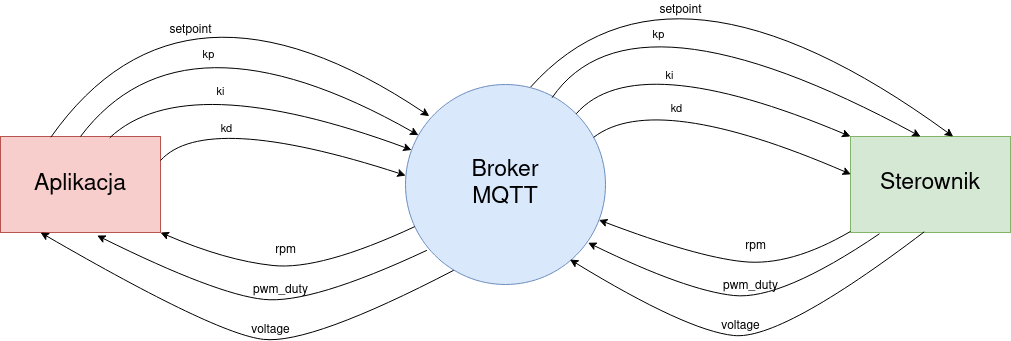
\includegraphics[width=1\textwidth]{img/dane.png}
      \caption{Schemat wymiany danych w systemie}
      \label{data_transmision}
    \end{figure}
 % schemat działania projektu

       
\chapter{Szczegółowy opis aplikacji dostępowej}
    \section{Grupa docelowa}
        Aplikacja okienkowa została stworzona, aby zwiększyć dostępność systemu dla osób nie wprawionych w tematy związane z protokołem MQTT. Istnieje pełen przekrój uniwersalnych aplikacji zdolnych do komunikacji za pośrednictwem owego protokołu. Część z nich świetnie naddawałaby się do kooperowania z resztą przygotowanego systemu. Z drugiej strony wszystkie tego typu aplikacje są zazwyczaj nad wyraz rozbudowane oraz wymagają od użytkownika pewnej specyficznej wiedzy i doświadczenia. Z tego też powodu w ramach projektu powstała aplikacja dedykowana opisywanemu systemowi. Gwarantuje ona kompatybilność z resztą elementów zawartych w projekcie jednocześnie posiadając opcje w pełni wykorzystujące wszystkie funkcjonalności systemu. Należy także dodać że projektowana była z myślą o prostocie, intuicyjności w obsłudze i minimalizmie.
        
    \section{Wykorzystana technologia}
        Sprostanie założeniom projektu jest trudnym zadaniem bazując jedynie na standardowych bibliotekach języka C++, ponieważ jednym z kluczowych aspektów projektu jest wykonanie zaawansowanej aplikacji okienkowej. Z tego powodu podjęta została decyzja o wykorzystaniu wysokopoziomowego frameworka, który znacząco uprościłby rozwój oprogramowania. Przykładem takiego rozwiązania jest bardzo popularny i nowoczesny framework QT. Jego niekomercyjna wersja jest w pełni darmowa i dystrybuowana na licencji otwarto źródłowej. Jego głównym przeznaczeniem jest tworzenie niezwykle rozbudowanych aplikacji okienkowych niewielkim nakładem pracy. Wspiera ono pełen przekrój systemów operacyjnych oraz architektur sprzętowych dzięki czemu program opierający się o tą technologię może być z powodzeniem przenoszony na różne urządzenia. Zdecydowanie najciekawszym aspektem tego oprogramowania jest niecodzienny system sygnałów i slotów. Według wielu początkujących programistów jest on nieintuicyjny. Jednakże wraz z korzystaniem z tego rozwiązania i towarzyszącym temu rosnącym doświadczeniem, pogląd ten jest niejednokrotnie rewidowany.  
        
        Poniżej przedstawione jest kilka fragmentów kodu użytego przy budowie aplikacji dostępowej wraz z opisami objaśniającymi wszystkie znajdujące się w nim zawiłości. % MQTT - opis
    
       
\chapter{Szczegółowy opis aplikacji dostępowej}
    \section{Grupa docelowa}
        Aplikacja okienkowa została stworzona, aby zwiększyć dostępność systemu dla osób nie wprawionych w tematy związane z protokołem MQTT. Istnieje pełen przekrój uniwersalnych aplikacji zdolnych do komunikacji za pośrednictwem owego protokołu. Część z nich świetnie naddawałaby się do kooperowania z resztą przygotowanego systemu. Z drugiej strony wszystkie tego typu aplikacje są zazwyczaj nad wyraz rozbudowane oraz wymagają od użytkownika pewnej specyficznej wiedzy i doświadczenia. Z tego też powodu w ramach projektu powstała aplikacja dedykowana opisywanemu systemowi. Gwarantuje ona kompatybilność z resztą elementów zawartych w projekcie jednocześnie posiadając opcje w pełni wykorzystujące wszystkie funkcjonalności systemu. Należy także dodać że projektowana była z myślą o prostocie, intuicyjności w obsłudze i minimalizmie.
        
    \section{Wykorzystana technologia}
        Sprostanie założeniom projektu jest trudnym zadaniem bazując jedynie na standardowych bibliotekach języka C++, ponieważ jednym z kluczowych aspektów projektu jest wykonanie zaawansowanej aplikacji okienkowej. Z tego powodu podjęta została decyzja o wykorzystaniu wysokopoziomowego frameworka, który znacząco uprościłby rozwój oprogramowania. Przykładem takiego rozwiązania jest bardzo popularny i nowoczesny framework QT. Jego niekomercyjna wersja jest w pełni darmowa i dystrybuowana na licencji otwarto źródłowej. Jego głównym przeznaczeniem jest tworzenie niezwykle rozbudowanych aplikacji okienkowych niewielkim nakładem pracy. Wspiera ono pełen przekrój systemów operacyjnych oraz architektur sprzętowych dzięki czemu program opierający się o tą technologię może być z powodzeniem przenoszony na różne urządzenia. Zdecydowanie najciekawszym aspektem tego oprogramowania jest niecodzienny system sygnałów i slotów. Według wielu początkujących programistów jest on nieintuicyjny. Jednakże wraz z korzystaniem z tego rozwiązania i towarzyszącym temu rosnącym doświadczeniem, pogląd ten jest niejednokrotnie rewidowany.  
        
        Poniżej przedstawione jest kilka fragmentów kodu użytego przy budowie aplikacji dostępowej wraz z opisami objaśniającymi wszystkie znajdujące się w nim zawiłości. % ESP - opis
        \section{Licznik impulsów}
        \subsection{Opis}
            Licznik impulsów (Pulse Counter) jest peryferium, które ułatwia obsługę enkoderów. Procesory bez takich udogodnień są skazane na odczytywanie przerwania za każdym razem jak enkoder wyśle impuls, aby następnie za pomocą kodu Graya rozpoznawać kierunek obrotu \cite{gray}. W takim zastosowaniu użycie enkodera jako pokrętła jest zrozumiałe. Zmieniając enkoder ręczny na taki zamontowany na silniku znacznie zwiększamy częstość generowania impulsów, a co za tym idzie również przerwań, odbieranych w sekundzie pracy procesora. W przypadku użytego w tym projekcie silnika prędkość obrotowa silnika przed przekładnią równa jest:
            
            \begin{displaymath}
              V = \frac{ n \cdot k}{t_{n}} = \frac{ 300 RPM \cdot 20.4 }{60s} = 102 RPS
            \end{displaymath}
            
            Gdzie:
            \begin{itemize}
                \item $n$ - ilość obrotów silnika za przekładnią w ciągu minuty pracy,
                \item $k$ - współczynnik redukcji przekładni,
                \item $t_{n}$ - okres czasu z którego brane są impulsy.
            \end{itemize}
            
            Wiedząc że zintegrowany enkoder generuje 11 impulsów na każdy obrót, zatem procesor zostanie będzie musiał obsłużyć 1122 przerwań w ciągu zaledwie jednej sekundy pracy. Taka kolej rzeczy z pewnością odbiłaby się na wydajności urządzenia. W ekstremalnym przypadku użycie większego silnika lub dokładniejszego enkodera mogłoby doprowadzić do sytuacji, gdzie procesor nie byłby w stanie obsłużyć tak dużej ilości przerwań. Rozwiązaniem tego problemu jest użycie liczników impulsów, które odciążają mikrokontrolery z takich wyzwań. Posiadają one swoją pamięć w której gromadzą dane na temat zliczonych sygnałów. W takiej sytuacji zadaniem procesora jest jedynie czytanie z tej pamięci. ESP32 posiada aż 8 takich liczników, co stwarza ogromne możliwość wykorzystania tego układu.
            
            Producent układu w dokumentacji procesora informuje że minimalny okres pomiędzy impulsami, który gwarantuje nie pominięcia żadnego odczytu nie może być mniejszy jak $12.5ns$. Wykorzystany w projekcie silnik obraca się z prędkością 100 obrotów na sekundę, a przy każdym obrocie enkoder produkuje 11 impulsów. Częstotliwość występowania impulsów jest następująca:
            
            \begin{displaymath}
              f = \frac{ n }{t_{n}} = \frac{ 100 \cdot 11 }{1s} = 1100Hz
            \end{displaymath}
            
            Gdzie $n$ oznacza generowaną ilość impulsów przez enkoder w okresie czasu $t_{n}$. Okres pomiędzy impulsami jest odwrotnością częstotliwości:
            
            \begin{displaymath}
              T = \frac{1}{ f } = \frac{1}{ 1100Hz } = 909.09 us
            \end{displaymath}
            
            Obliczenia zostały poparte pomiarami z oscyloskopu. Pomiar został umieszczony na rys. \ref{fig:pcnt_osc}. Widać na nim że częstotliwość waha się w okolicy 1040Hz. Delikatne zwiększenie napięcia zasilania spowodowałoby minimalny wzrost obrotów, więc uzyskanie wyliczonej częstotliwości nie jest problemem. Niemniej jednak, okres pomiędzy impulsami enkodera jest o rzędy wielkości większy niż okres graniczny dla tego licznika. Oznacza to że można wypełni ufać wskazaniom licznika ponieważ że żadne impulsy nie są pomijane.
            Abstrahując od okresów pomiędzy impulsami obraz z oscyloskopu wspaniale prezentuje przesunięcie przebiegów pomiędzy kanałami enkodera. 
            
            
            \begin{figure}[ht]
                \centering
                \includegraphics[width=0.9\textwidth]{img/counter_period.png}
                \caption{Pomiar impulsów z oscyloskopu}
                \label{fig:pcnt_osc}
            \end{figure}
            
            
            
            
        \subsection{Konfiguracja}
            W przypadku tego układu, konfiguracja jest bardzo prosta i sprowadza się do wypełnienia zaledwie dwóch struktur i wysłania ich do peryferium.
            
            \begin{kod}
              \inputminted[firstline=5,lastline=48]{cpp}{esp/listings/encoder_driver.cpp}
              \caption{Konfiguracja licznika impulsów}
              \label{code:pcnt}
              \vspace{2em}
            \end{kod} 
            
            Użycie jednej struktury powoduje włączenie jednego z dwóch kanałów w liczniku. Licznik automatycznie ewaluuje zbocza narastające na obu wyjściach enkodera, co podwaja wykrywaną ilość impulsów. Poprawne skonfigurowanie obu kanałów w liczniku w sposób pokazany na listingu \ref{code:pcnt} sprawia że licznik poprzez analizę zbocz narastających jak i opadających zwiększa dokładność enkodera aż czterokrotnie. Opisane rozwiązanie sprawiło że użyty w projekcie tani enkoder dostarcza aż 897 impulsów na każdy obrót wału wyjściowego z przekładni. Skutkuje to impulsem co około 0.4°. Proces ten został opisany w publikacji \cite{enkoder}. Poza konfiguracją licznika wystarczy jedynie dbać o odczyt zliczonych impulsów oraz zerowanie pamięci po wykonanym odczycie. Funkcje odpowiedzialne za te czynności zostały przedstawione w listingu \ref{code:encoder_macro}. % ESP - licznik
        \section{Modulacja szerokości impulsu - PWM} 
        \subsection{Opis}
            Najpopularniejszym sposobem sterowania silnikami prądu stałego jest wykorzystanie metody PWM \cite{pwm} czyli modulacji szerokości impulsu. Cechuje się ona tym że nie wymaga użycia skomplikowanych przetworników cyfrowo-analogowych, jednocześnie umożliwiając płynne sterowanie mocą elementów takich jak diody czy silniki. Jej działanie polega na bardzo szybkim przełączaniu pomiędzy stanami wysokim i niskim. Im dłuższy okres czasu zajmuje stan wysoki w cyklu pracy regulatora, tym więcej energii dostarczane jest do sterowanego elementu. Stosunek tego okresu do okresu pracy PWM nazywany jest wypełnieniem. Przebiegi przy trzech różnych wypełnieniach zostały przedstawione na obrazku \ref{fig:pwm_duty}.
            
            \vspace{1em}
                                
            \begin{figure}[ht]
                \centering
                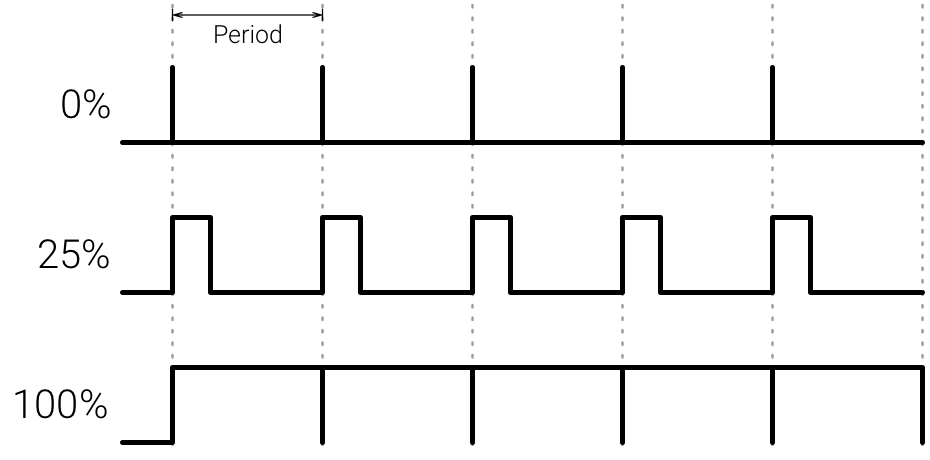
\includegraphics[width=1\textwidth]{img/pwm-duty.png}
                \caption{Przebieg modulacji PWM \cite{pwm_fig}}
                \label{fig:pwm_duty}
            \end{figure}
            
            \vspace{1em}
        
        
        \subsection{Implementacja}
            Za obsługę peryferium PWM odpowiada klasa "Motor" przedstawiona w listingu \ref{code:pwm_init}. Utworzenie obiektu tej klasy automatycznie inicjalizuje peryferium odpowiedzialne na obsługę PWM. Wybór częstotliwości pracy był podyktowany minimalizacją hałasu generowanego podczas pracy silnika. Z tego powodu zdecydowano się na wartość 22kHz, czyli granice ludzkiego słuchu. Jest to także typowa wartość proponowana przez producenta użytego mostka H \cite{mostek}.
            
            Peryferium znajdujące się w wykorzystanym układzie pozwala na generowanie symetrycznego PWM. Różni sie ono od tradycyjnej asymetryczenej regulacji tym że generowane impulsy są zawsze symetryczne względem środka. Zaletą takiego rozwiązania jest generowanie mniejszych harmonicznych w napięciach i prądach wyjściowych oraz lepiej naddaje się ono do sterowania silnikami DC \cite{pwm_center}. Porównanie przebiegów symetrycznego i asymetrycznego PWM zostało umieszczone na obrazku \ref{fig:sym_pwm}
            
            \begin{figure}[ht]
                \centering
                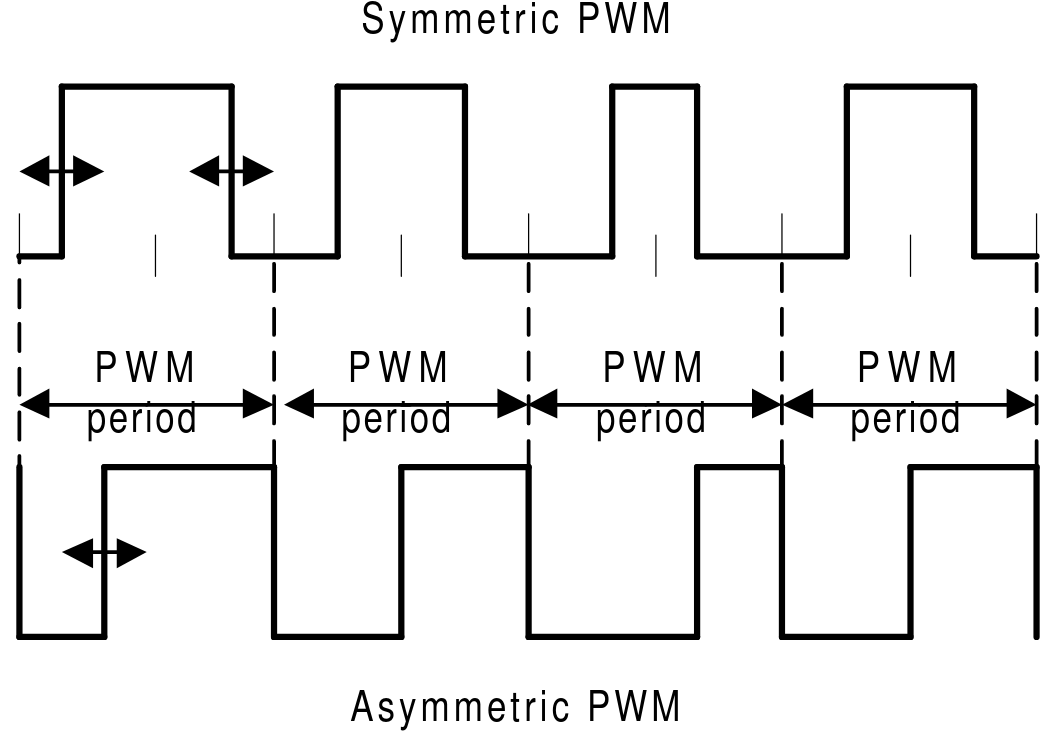
\includegraphics[width=0.9\textwidth]{img/symetric_pwm.png}
                \caption{Przebieg modulacji PWM \cite{pwm_center}}
                \label{fig:sym_pwm}
            \end{figure}   
            
            
        \begin{kod}
          \inputminted[firstline=3,lastline=24]{cpp}{esp/listings/motor_driver.cpp}
          \caption{Inicjalizacja PWM}
          \label{code:pwm_init}
          \vspace{1em}
        \end{kod}
        
        Jedyna metoda tej klasy wykorzystywana podczas typowej pracy programu jest przedstawiona na listingu \ref{code:pwm_duty}. Jej zadaniem jest zmiana ustawień wypełnienia PWM oraz kierunku obrotu silnika w zależności od przekazanej wartości.
        
        \begin{kod}
          \inputminted[firstline=27]{cpp}{esp/listings/motor_driver.cpp}
          \caption{Zmiana wypełnienia PWM}
          \label{code:pwm_duty}
          \vspace{2em}
        \end{kod} % ESP - PWM
        \section{Regulator PID} 
    
    \subsection{Implementacja}
         Najważniejszą częścią programu jest implementacja regulatora PID. Odpowiednie zaprojektowanie jego działania jest kluczowe w kwestii wydajności oraz poprawności funkcjonowania całego systemu \cite{hor}. Schemat funkcjonowania algorytmu jest prosty i został on przedstawiony na listingu \ref{code:pid_compute}.
         
         Pierwszym krokiem jest odczytanie z rejestru licznika ilości zliczonych impulsów. Następnie należy wyzerować ten rejestr, aby mógł on ponownie zliczać kolejne impulsy zaczynając od zera. Operacja ta musi zostać wykonana bezpośrednio po dokonaniu odczytu, aby nie pominąć żadnych impulsów, które będą pojawiać się w trakcie wykonywania dalszych obliczeń. Realizacja tego krótkiego procesu przesłonięta przez marko zawarte w \ref{code:encoder_macro} w celu zwiększenia czytelności kodu. 
         
        \begin{kod}
          \inputminted[firstline=10,lastline=12]{cpp}{esp/listings/encoder_driver.hpp}
          \caption{Pobieranie wartości i czyszczenie rejestrów licznika}
          \label{code:encoder_macro}
          \vspace{1em}
        \end{kod}
         
         
         Warto zaznaczyć że nie jest zapisywany moment pobrania danych. Musi więc być zagwarantowane że funkcja wykonująca odczyt będzie wykonywać się cyklicznie w ściśle określonym przedziale czasowym. Każde odstępstwo od tego będzie powodowało błędy w poprawnym działaniu algorytmu. 
         
        \begin{kod}
          \inputminted[firstline=17,lastline=45]{cpp}{esp/listings/pid.cpp}
          \caption{Pętla regulatora PID}
          \label{code:pid_compute}
          \vspace{2em}
        \end{kod}
    
         Kolejnym krokiem jest wyliczenie uchybu regulacji i jest to tradycyjnie różnica wartości ustalonej i zliczonych impulsów. Następnie liczymy wartości dla każdego z członów regulacji, jednocześnie gwarantując że mieszczą się one we wcześniej zdefiniowanych przedziałach. To również ukryte zostało pod makrem dostępnym w listingu \ref{code:pid_macro}.
         
         Wartości każdego z członów mnożymy poprzez wybrane przez użytkownika współczynniki. Są one zapisane w zmiennych dzięki czemu istnieje możliwość zmiany ich wartości dynamicznie podczas pracy programu. Teraz wystarczy już zsumować wszystkie wartości oraz zapewnić że uzyskana wartość nie przekroczy wartości granicznych możliwych do ustawienia dla PWM. W tym momencie część obliczeniowa jest gotowa. Istnieje jednak spore ryzyko że uzyskana w ten sposób wartość nie będzie mieściła się w zakresie przyjmowanym przez peryferium odpowiedzialnym za modulowanie napięcia. Niezbędne jest więc wykonanie kolejnej normalizacji do akceptowalnych wartości  \ref{code:pid_macro}. 
       
        \begin{kod}
          \inputminted[firstline=10,lastline=16]{cpp}{esp/listings/pid.hpp}
          \caption{Normalizacja wartości regulatora}
          \label{code:pid_macro}
          \vspace{1em}
        \end{kod}
    
    \subsection{Proces PID}
        Pętla regulatora PID zaimplementowana jest w swoim własnym procesie. Ułatwia to kontrolę częstości wykonywania obliczeń i umożliwia zatrzymanie procesu gdy jest on niepotrzebny. Na przykład przy braku połączenia z serwerem MQTT.
        
        Implementacja procesu zawarta jest w listingu \ref{code:pid_task}. Pierwsze linie kodu rozpoczynają inicjalizację niezbędnych obiektów. W skład nich wchodzi:
        
        \begin{itemize}
            \item config - struktura zawierająca konfigurację parametrów regulatora. Niezbędna do dynamicznej zmiany parametrów PID.
            
            \item engine - instancja sterująca peryferium PWM,
            \item encoder - instancja do obsługi enkodera,
            \item pid - instancja regualtora PID,
            \item pid\_result - zmienna zawirająca wyliczoną wartość regulacji,
        \end{itemize}
        
        Kolejne linie kodu wykonują się w nieskończonej pętli. Następuje w niej odczyt aktualnego stanu licznika systemowego. Jest on wykorzystywany do wyliczenia jak długo wykonują się operacje w pętli. Następnie sprawdzana jest kolejka FIFO. W przypadku znalezienia się w niej nowej konfiguracji dla regulatora, jest ona natychmiast zastosowana. 
        
        \begin{kod}
          \inputminted[firstline=58]{cpp}{esp/listings/pid.cpp}
          \caption{Proces wykonywanie PID}
          \label{code:pid_task}
          \vspace{2em}
        \end{kod}
        
        Po opuszczeniu instrukcji warunkowej następuje obliczenie wartości regulatora i ustawienie modulacji szerokości impulsu zgodnie z uzyskanym wynikiem. Ostatnim krokiem jest zatrzymanie procesu. Czas zatrzymania jest zależny od prędkości wykonywania pętli i warunkuje częstotliwość wyzwalania PID na 100Hz. Na obrazku \ref{fig:pid_plantuml} znajduje się diagram aktywności opisywanego procesu.
        
                      
        \begin{figure}[ht]
            \centering
            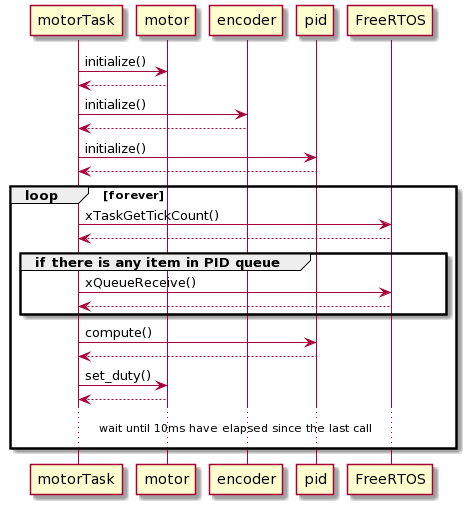
\includegraphics[width=0.8\textwidth]{img/motorTask_uml.png}
            \caption{Diagram aktywności procesu PID}
            \label{fig:pid_plantuml}
        \end{figure} % ESP - PID
        \section{Pomiar napięcia}
         Pomiar napięcia dokonywany jest przy użyciu przetwornika analogowo-cyfrowego wbudowanego w mikroprocesor \cite{esp32}. Posiada on bowiem dwa 12 bitowe przetworniki, których wejścia są multipleksowane na aż 18 pinów. Po wczytaniu się w dokumentację okazuje się jednak że użyteczność tych przetworników ma wiele wykluczeń. Najważniejszym z nich jest interferencja przetwornika ADC2 z peryferium odpowiedzialnym za połączenie WiFi. Oznacza to że w projektach od których wymagamy stałego połączenia z siecią jesteśmy ograniczeni jedynie do 8 pinów obsługujących odczyty analogowe. 
         
         Kolejnym ciekawym aspektem tego układu jest możliwość programowego wyboru tłumienia sygnału wejściowego. Producent umożliwia nam wybór od 0dB poprzez 2.5dB oraz 6dB aż do 11dB tłumienia. Im wyższy parametr zostanie wybrany tym wyższe napięcia jest w stanie obsłużyć przetwornik. Niemniej jednak wybór wyższych oczek znacznie degraduje precyzję pomiaru.
     
     
    \subsection{Konfiguracja ADC}
        Po dokładnym przestudiowaniu dokumentacji przyjęte zostało ustawienie tłumienia na poziomie 2,5dB. Patrz \ref{code:adc1}. Wyższe ustawienia wprowadzają znaczną niedokładność pomiarów. Według dokumentacji \cite{esp32} takie ustawienie sprawia że efektywny zakres pomiarowy kształtuje się w zakresie od 100mV do 1250mV na pinie mikrokontrolera. Błędy pomiaru zadeklarowane przez producenta nie powinny przekroczyć $ \pm 30 mV$. Jednakże, zasilanie płytki jest zaprojektowane do obsługi dużo większych napięć, tak aby móc wykorzystywać szeroki zakres silników. Podanie napięcia wyższego jak zasilanie procesora, które w tym wypadku wynosi 3.3V, spowodowałoby trwałe uszkodzenia układu. Do bezpiecznego pomiaru napięcia zasilania niezbędne jest więc zastosowanie dzielnika napięcia. 
        
        Rozdzielczość peryferium została ustawiona na 12 bitów. Wynika z tego że istnieje $2^{12} = 4096$ poziomów kwantyzacji. Nie spodziewam się że mój autorski projekt płytki drukowanej \ref{fig:pcb} będzie miał na tyle niski szum kwantyzacji, aby móc w pełni wykorzystać taką rozdzielczość, ale w tym przypadku czas pomiaru nie jest tutaj kluczowy. Założenie wykonywania pomiaru zakłada że i tak będzie wykonywane wiele pomiarów pod rząd, aby później móc wyciągnąć z nich średnią.
        
        \begin{kod}
          \inputminted[firstline=8,lastline=17]{cpp}{esp/listings/adc.cpp}
          \caption{Konfiguracja przetwornika ADC}
          \label{code:adc1}
          \vspace{2em}
        \end{kod}
        

    

        
    \subsection{Dzielnik napięcia}
        Zadecydowałem że w tym projekcie wystarczający będzie najprostszy dzielnik oparty na dwóch rezystorach. Pozwoli nam on liniowo podzielić napięcie, tak aby nigdy nie przekroczyło ono wartości niebezpiecznej dla mikroprocesora. Do stworzenia dzielnika wykorzystałem rezystory z szeregu E24 \cite{szereg} o wartościach $9.1k \Omega $ oraz $1k \Omega $ i podłączyłem je w sposób pokazany na schemacie \ref{fig:pcb_schematic_1}.
        
        Obliczenie dostępnego zakresu pomiarowego przetwornika adc odbywa się przy pomocy wzoru na dzielnik napięcia \cite{dzielnik}. Jest on następujący:
        
        \vspace{1em}
        \begin{displaymath}
          V_{out} = \frac{ R_2 }{ R_1 + R_2 } \cdot V_{in}
        \end{displaymath}
        \vspace{1em}
        
        Gdzie napięcie wejściowe $V_{out}$ jest maksymalnym napięciem dostępnym na wejściu przetwornika. Zgodnie z informacją zawartą w dokumentacji procesora \cite{esp32} wybranie tłumienia na poziomie 2.5dB skutkuje otrzymaniem 1250mV jako granicy efektywnego zakresu pomiarowego. Przy czym producent zaznacza że ta wartość zależy od konkretnego egzemplarza i może się wahać. $R_1$ oraz $R_2$ to użyte rezystory w dzielniku. W tym przypadku są to kolejno $9.1k \Omega $ oraz $1k \Omega $.
        
        Dla maksymalnego obsługiwanego napięcia z przedziału wzór to:
        
        \vspace{1em}
        \begin{displaymath}
          1.250V = \frac{ 1k \Omega  }{ 9.1k \Omega  + 1k \Omega  } \cdot V_{in}
        \end{displaymath}
        \vspace{1em}
        
        Po przekształceniu go tak aby wyliczyć napięcie przed dzielnikiem otrzymujemy:
        
        \vspace{1em}
        \begin{displaymath}
         V_{in} = \frac{ 1.250V \cdot (9.1k \Omega  + 1k \Omega)  }{ 1k \Omega  } = 12.625 V
        \end{displaymath}
        \vspace{1em}
        
        Dla najniższego napięcia w mieszczącego się w zakresie efektywnego pomiaru (100mV) otrzymamy:
        
        \vspace{1em}
        \begin{displaymath}
         V_{in} = \frac{ 0.100V \cdot (9.1k \Omega  + 1k \Omega)  }{ 1k \Omega  } = 1.01 V
        \end{displaymath}      
        \vspace{1em}
        
        Oznacza to że w zakresie zasilania od $1.01V$ do $12.625V$ mamy dużą szansę uzyskać wynik pomiaru bliski rzeczywistemu.
        
    \newpage
        
    \subsection{Wyznaczanie współczynnika konwersji}
        W celu przeliczenia wartości odczytywanych z przetwornika analogowy-cyfrowego na napięcie wyrażone w woltach, niezbędne jest wyznaczenie współczynnika konwersji. 
        
        Posiadając wiedzę na temat użytych rezystorów w dzielniku napięcia, jest możliwe wyliczenie tego współczynnika. Aczkolwiek, moje doświadczenie z projektowaniem układów pomiarowych podpowiada że teoria bardzo często mija się z praktyką i zazwyczaj kalibruję swoje układy wykonując serię pomiarów. Tak też zrobiłem w tym przypadku. Wyniki zostały przedstawione na wykresie \ref{fig:adc_plot}
 
        \begin{figure}
        \vspace{1em}
            \centering
            \begin{tikzpicture}
                \centering
                \begin{axis}[ylabel = adc readings, xlabel = voltage, legend pos=north west, ymajorgrids=true, grid style=dashed, width=0.9\textwidth]
                    \addplot table [x=a, y=b, col sep=comma] {esp/adc_plot.dat};
                    \addlegendentry{\(ADC_{RAW}\)}
                    \addplot [domain=4.8:14.5, samples=100, color=red] {x*308 - 292};
                    \addlegendentry{\(x*308 - 292\)}
                \end{axis}
            \end{tikzpicture}
            \caption{Pomiary danych ADC do napięcia zasilania}
            \label{fig:adc_plot}
        \end{figure}
        \vspace{1em}
        
        %TODO dodać opis osi, jednostki, czerwoną linię regresji  
        
        Uzyskane pomiary potwierdzają że prawie cały zakres przetwornika, nie licząc końców, jest liniowy. Pomiary zakończyłem przy około $5.1V$ ponieważ poniżej tej wartości stabilizator liniowy, użyty do obniżenia napięcia na procesorze, przestawał poprawnie działać, co kończyło się resetami jednostki centralnej.
        
        Dzięki regresji liniowej byłem w stanie wyprowadzić równanie, które w łatwy sposób umożliwia przeliczanie odczytów z ADC na wartość napięcia.
        
        \vspace{1em}
        \begin{displaymath}
          y = \frac{ ADC_{RAW} + 292 }{ 398 }
        \end{displaymath}    
        \vspace{1em}
        
        Za $ADC_{RAW}$ wstawiamy wartość pomiaru i otrzymujemy napięcie wyrażone w woltach.
        
        
        
        
    \subsection{Rozdzielczość pomiaru}
        Posiadając już możliwość przeliczania surowych odczytów na napięcie, należałoby wyznaczyć rozdzielczość otrzymanych danych. Do obliczenia rozdzielczości napięciowej, czyli najmniejszego możliwego skoku zdolnego do zapisania przed przetwornik, musimy wykonać dwa pomiary. Następnie należy porównać różnice obliczonych napięć do różnicy surowych danych. Przy pomocy podanego wzoru:
        
        \vspace{1em}
        \begin{displaymath}
          \frac{ V_{1} - V_{2} }{ ADC_{1} - ADC_{2} } = \frac{ 10.136V - 6.171V  }{ 2826 - 1609 } = \frac{ 3.965V }{ 1217 } = 0.0032V
        \end{displaymath}    
        \vspace{1em}
          
          
    \subsection{Wykonywanie pomiarów}
        Wykonywanie pomiarów jest wykonywane na osobnym procesie. Dzięki temu można w łatwy sposób kontrolować częstotliwość mierzenia napięcia i wysyłania danych z ADC na MQTT. Pętla wyzwalająca odczyt wykonuje się raz na 20 milisekund. W każdej iteracji następuje pomiar, a odczytana wartość umieszczana jest w buforze. Co dziesiąta iteracja wylicza średnią z pomiarów, konwertuje wartość na wolty i wysyła dany na MQTT. Diagram aktywności umieszczony został w listingu \ref{fig:adc_plantuml}. 
        
 
        
        \begin{kod}
          \inputminted[firstline=19, lastline=44]{cpp}{esp/listings/adc.cpp}
          \caption{Wyzwalanie pomiaru i przeliczanie wartości}
          \label{code:adc2}
          \vspace{2em}
        \end{kod}
        
        
        \begin{figure}[ht]
          \centering
          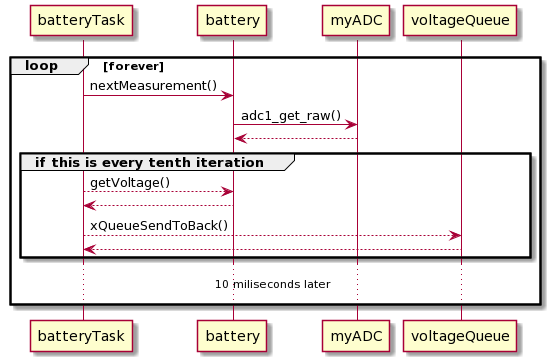
\includegraphics[width=0.8\textwidth]{img/adc_uml.png}
          \caption{Diagram aktywności dokonywania pomiarów}
          \label{fig:adc_plantuml}
        \end{figure}
 
        
        
        
        
        % 1000 i 9100
        % 1021 i 9273
        % y = 308*x -292
        % x = y+292 / 308
        
        
         % ESP - adc
        \section{Łączenie z brokerem MQTT}
        Jedną z zalet wykorzystania oficjalnego frameworka wydawanego przez producenta jest gotowa implementacja warstw abstrakcji ułatwiających obsługę protokołu MQTT. Umożliwia ona łatwą konfigurację i wykorzystanie tego środka komunikacji za pomocą kilku wysokopoziomowych funkcji.
        
        \subsection{Konfiguracja}
        Pierwsze co należy zrobić to wypełnić strukturę konfiguracyjną, w której znajduje się aż 165 elementów. Jednak dla prawidłowej pracy wystarczy wypełnić kilka podstawowych pól takich jak dane logowania użytkownika czy adres brokera. Część z nich służy jako wskaźniki do danych przychodzących, bufory, czy flagi niezbędne do funkcjonowania. 
        
        Kolejnym krokiem jest stworzenie struktury inicjalizacyjnej przy pomocy poprzedniej struktury. Posłuży nam do tego specjalna funkcja która sprawdza poprawność wprowadzonych przez nas danych, a dane nie definiowane zostają zastąpione wartościami domyślnymi. 
        
        Następne musimy wybrać jakie zdarzenia chcemy rejestrować i gdzie mają one trafiać. W tym przypadku wybieramy pełną pulę dostępnych sygnałów. Zawartość funkcji obsługującej zdarzenia znajduje się w listingu \ref{code:mqtt5}. 
        
        Pozostaje już tylko uruchomić moduł MQTT przekazując powstałą konfigurację do funkcji startowej. Dane zostaną przesłane do nowego procesu, który zajmie się za nas obsługą komunikacji. Wszystkie niezbędne kroki oraz konfiguracja została przedstawiona na listingu \ref{code:mqtt1}. 
        
        \begin{kod}
            \inputminted[firstline=130]{cpp}{esp/listings/mqtt.cpp}
            \caption{Konfiguracja połączenia MQTT}
            \label{code:mqtt1}
            % \vspace{2em}
        \end{kod}
        
        
        
        \subsection{Obsługa zdarzeń}
        Wykorzystana warstwa abstrakcji posiada system udostępniający nam możliwość odbierania sygnałów generowanych przez zdarzenia wynikające z pracy klienta MQTT. Skorzystamy z tej funkcjonalności, aby informować użytkownika o stanie komunikacji, a także aby odpowiednio reagować na zdarzenia. Została ona załączona w listingu \ref{code:mqtt5}.
        
        Po otrzymaniu sygnału poprawnego nawiązania połączenia, zaczynamy subskrybować wszystkie tematy które przechowują potrzebne nam dane. Jest to przedstawione na listingu \ref{code:mqtt3}.
          
        \begin{kod}
            \inputminted[firstline=14, lastline=19]{cpp}{esp/listings/mqtt.cpp}
            \caption{Subskrybowanie niezbędnych tematów}
            \label{code:mqtt3}
            \vspace{1em}
        \end{kod}
        
        
        
        Kolejnym krokiem jest utworzenie nowego procesu przypisanego do rdzenia drugiego (numeracja jest od zera). Jego zadaniem jest transmisja danych z urządzenia do brokera. Utworzenie kolejnego zadania oraz sam fakt pomyślnego uzyskania połączenia obarczony jest komunikatem diagnostycznym.
        
        Otrzymanie informacji o zakończeniu połączenia wiąże się z odwróceniem zmian dokonanych przez poprzedni sygnał. Po wysłaniu komunikatu na strumień wyjścia, dokonujemy zabicia procesu wysyłającego dane, po uprzednim sprawdzeniu czy taki jeszcze istnieje. Jest to zabezpieczenie przez sytuacją, gdy istnieje więcej jak jeden taki proces. Następnie po odczekaniu jednej sekundy, wyzwalana jest próba ponownego łączenia. 
        
        Ostatnim ważnym sygnałem jest informacja o zmianie wartości subskrybowanego kanału. Jest ona obrazu  przekazywana do stworzonej prze zemnie funkcji. Znajduje się ona w listingu \ref{code:mqtt4}. Jej jedynym zadaniem jest dodawanie odebranych wartości do odpowiednich kolejek priorytetowych w zależności od tematu wiadomości. 
     
        \begin{kod}
            \inputminted[firstline=21, lastline=44]{cpp}{esp/listings/mqtt.cpp}
            \caption{Odbieranie danych}
            \label{code:mqtt4}
            \vspace{1em}
        \end{kod}
        
           
           
        Pozostałe sygnały służą czysto w celach diagnostycznych. Z tego też powodu nie wykonują one żadnego kodu poza raportowaniem zdarzenia poprzez komunikat na standardowym strumieniu wyjścia.  
        
        \begin{kod}
            \inputminted[firstline=73, lastline=125]{cpp}{esp/listings/mqtt.cpp}
            \caption{Obsługa sygnałów}
            \label{code:mqtt5}
            \vspace{2em}
        \end{kod}
        
        

        \subsection{Wysyłanie danych}
        Transmisja informacji odbywa się na osobnym procesie aniżeli reszta modułu MQTT. Logika przekazywania danych jest względnie prosta. Wystarczy odebrać wiadomość z kolejki priorytetowej, a następnie przekazać ją do wysłania z pomocą odpowiedniej funkcji. Na listingu \ref{code:mqtt6} przedstawione jest wysyłanie wiadomości na wszystkich trzech tematach zarządzanych przez mikrokontroler.
        
        \begin{kod}
            \inputminted[firstline=46, lastline=71]{cpp}{esp/listings/mqtt.cpp}
            \caption{Wysyłanie danych}
            \label{code:mqtt6}
            \vspace{2em}
        \end{kod} % ESP - mqtt
    \section{Gotowe urządzenie}

    \subsection{Symulacja}
    Symulacje gotowego urządzenia zostały przedstawione na rysunkach \ref{fig:prototype_sym_1} oraz \ref{fig:prototype_sym_2}.
    
    \begin{figure}[ht]
        \centering
        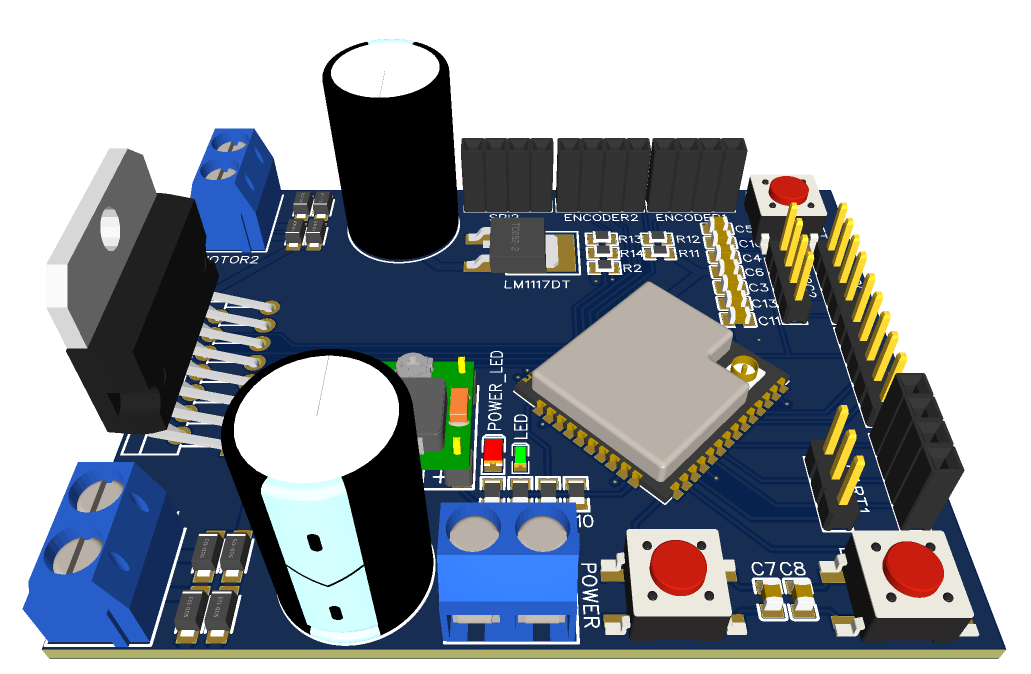
\includegraphics[height=0.32\textheight]{img/prototype_sym_1.png}
        \caption{Symulacja  gotowego urządzenia (wierzch)}
        \label{fig:prototype_sym_1}
    \end{figure}
    
    \begin{figure}[ht]
        \centering
        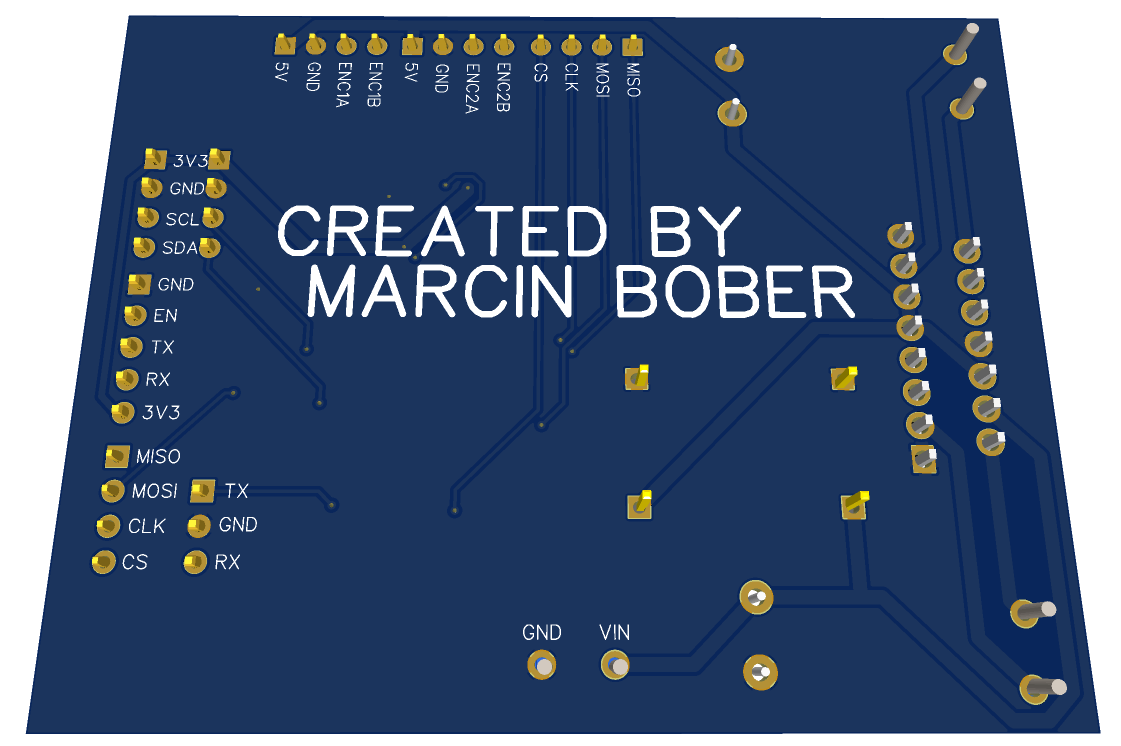
\includegraphics[height=0.32\textheight]{img/prototype_sym_2.png}
        \caption{Symulacja gotowego urządzenia (spód)}
        \label{fig:prototype_sym_2}
    \end{figure}

    
    \subsection{Prototyp}
    Zdjęcia  gotowego urządzenia zostały przedstawione na rysunkach \ref{fig:prototype_real_1} oraz \ref{fig:prototype_real_2}.
    
    \begin{figure}[ht]
        \centering
        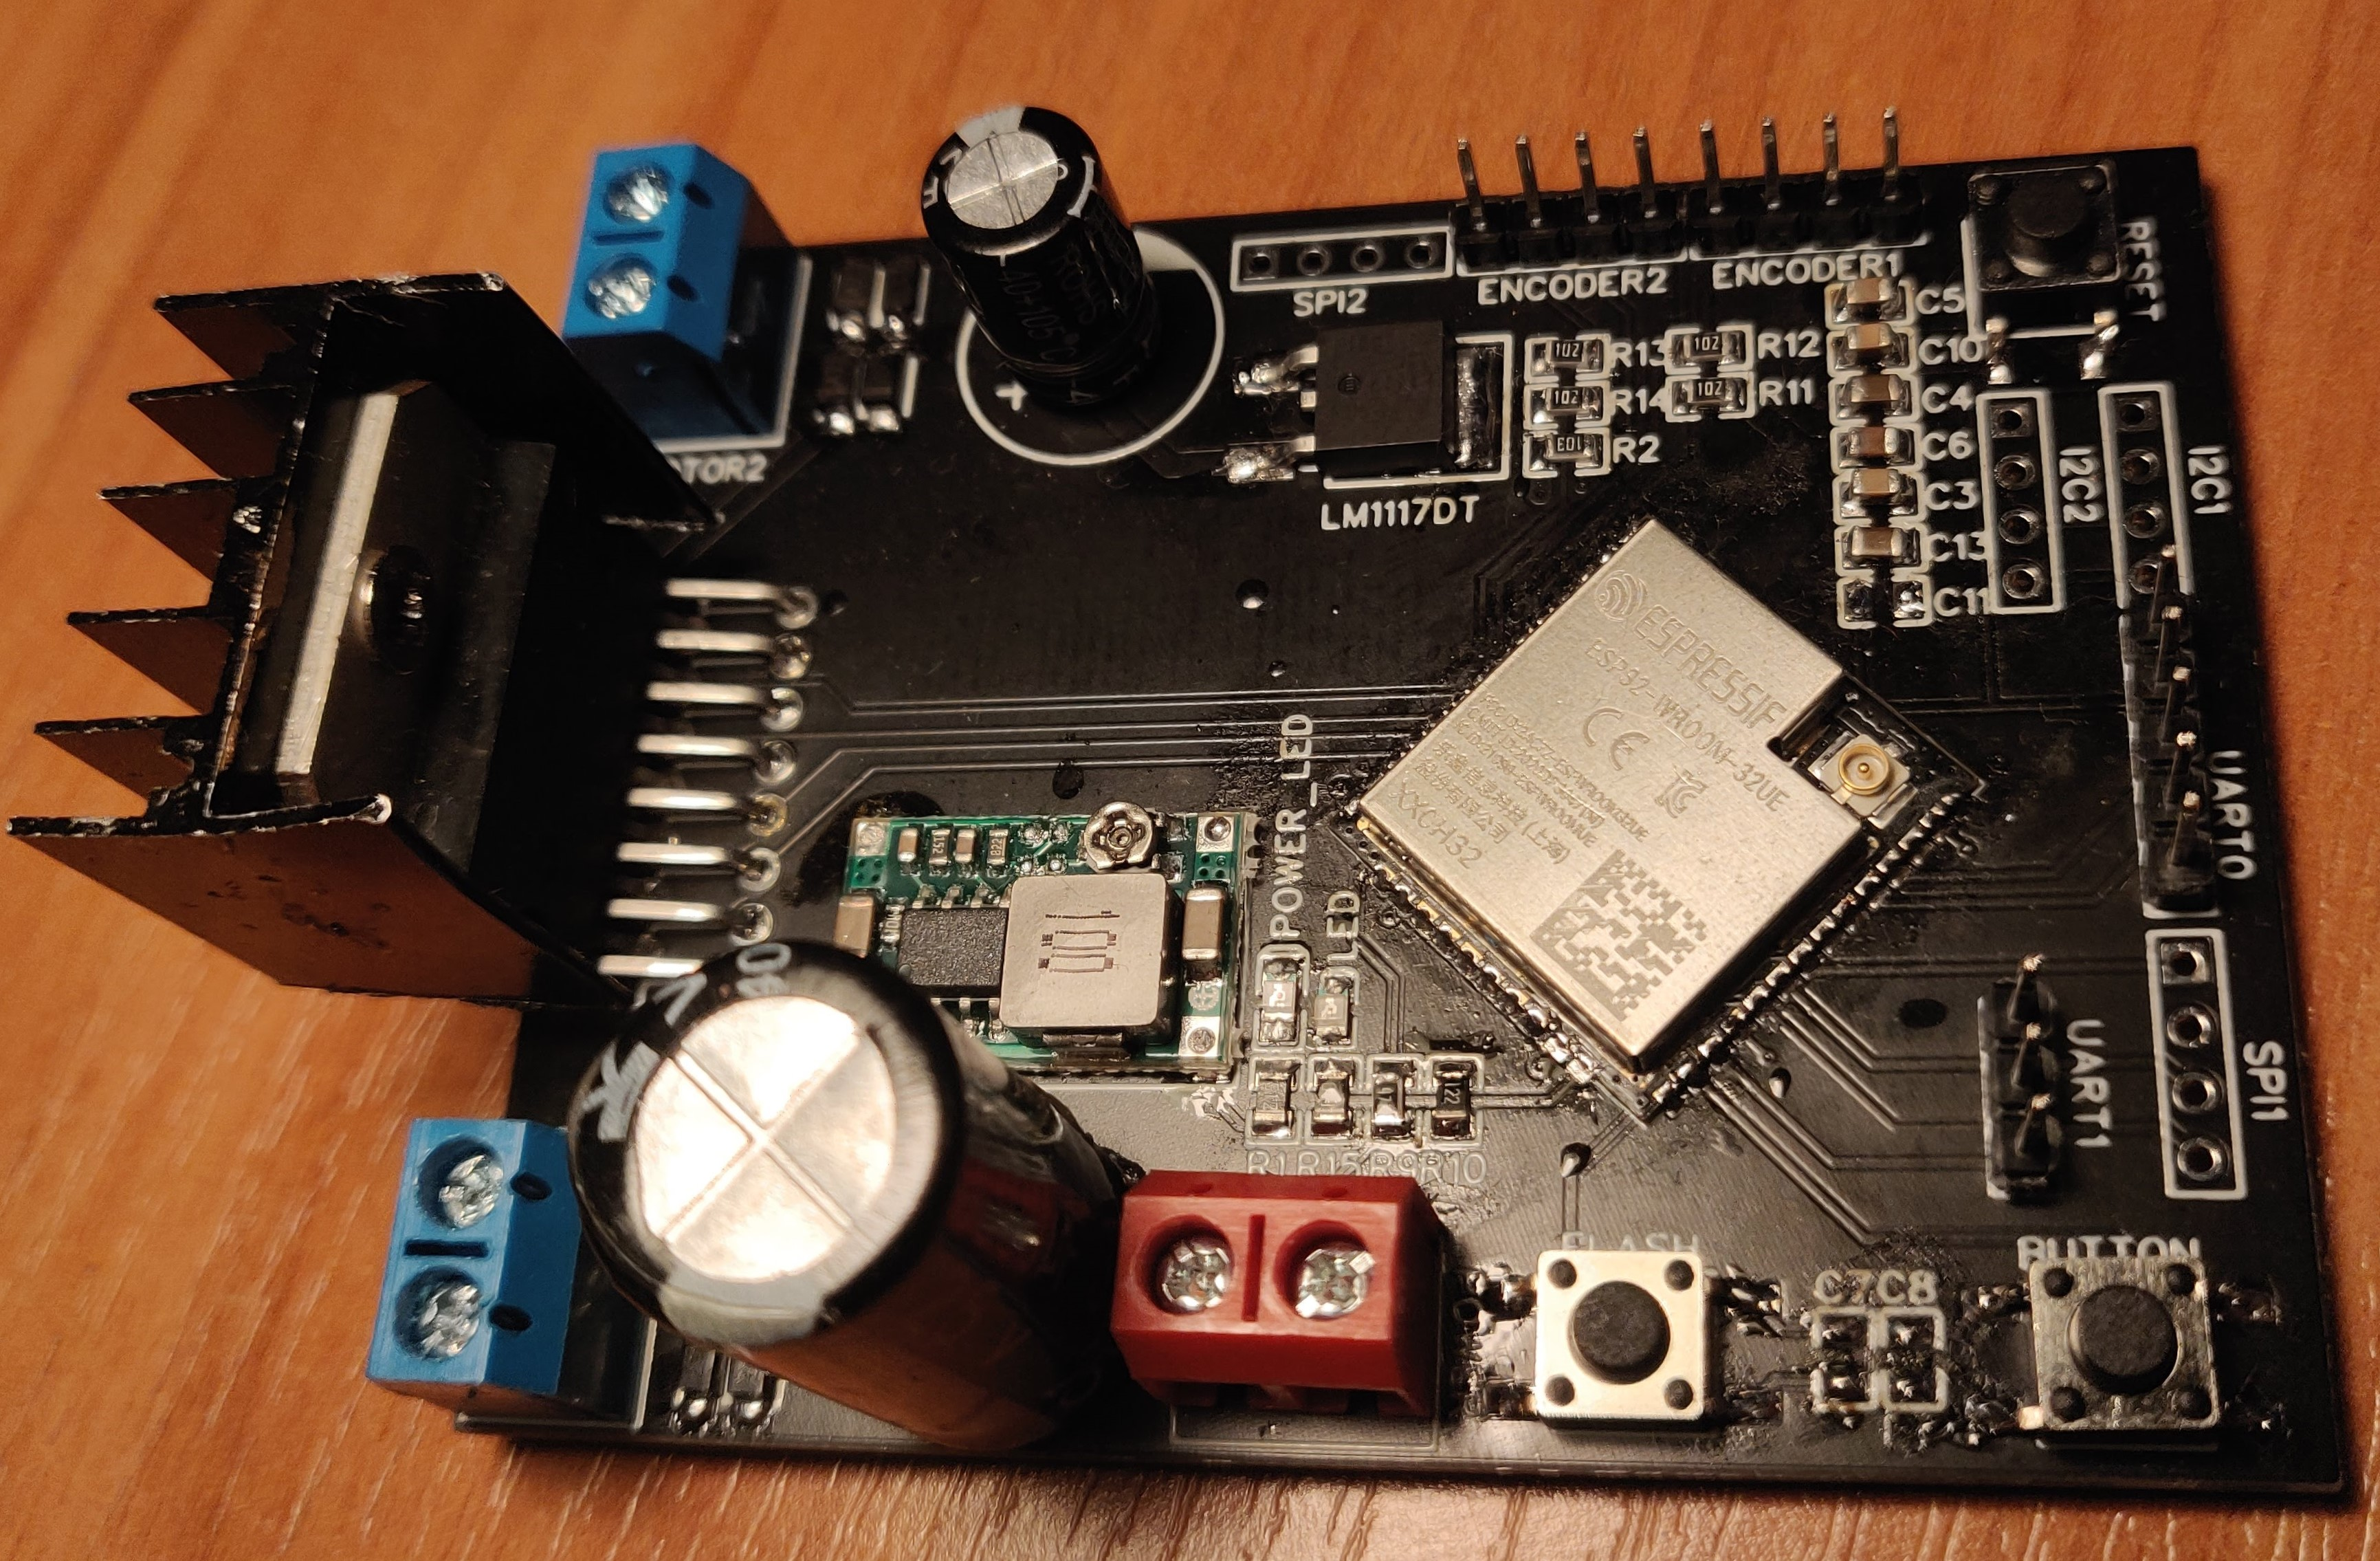
\includegraphics[height=0.4\textheight]{img/prototype_real_1.jpg}
        \caption{Zdjęcie gotowego urządzenia (wierzch)}
        \label{fig:prototype_real_1}
    \end{figure}
    
    \begin{figure}[ht]
        \centering
        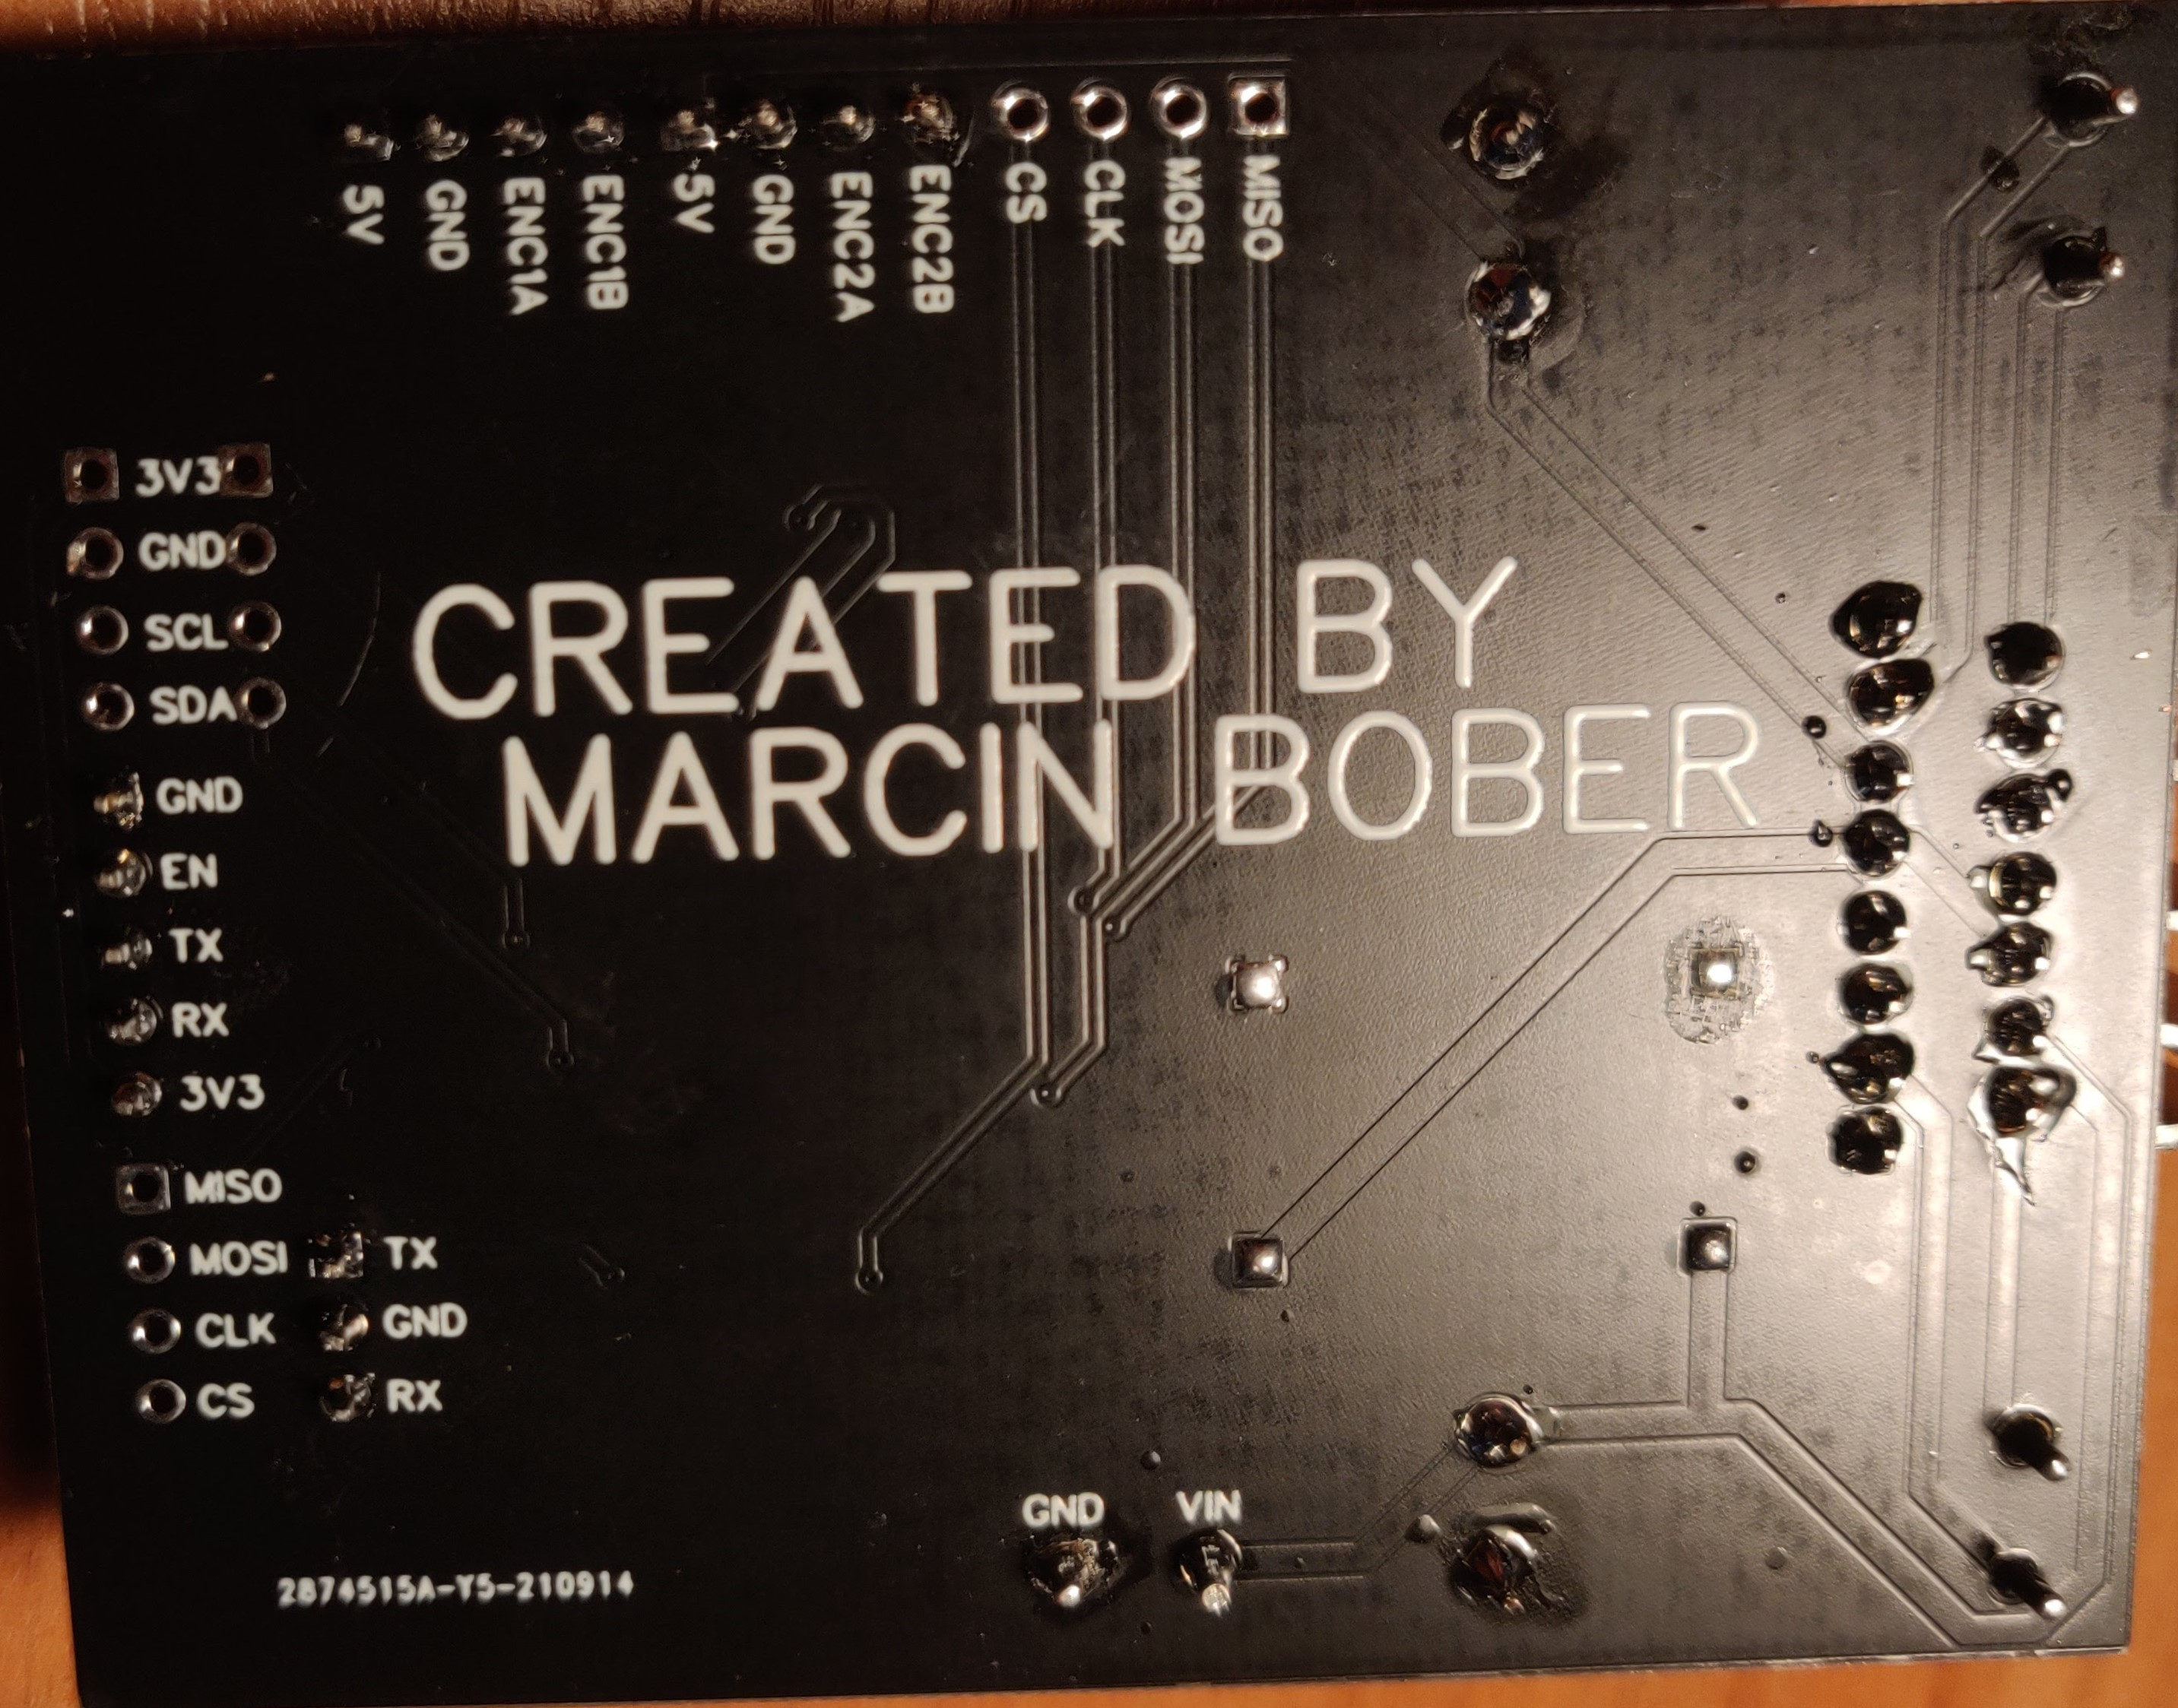
\includegraphics[height=0.45\textheight]{img/prototype_real_2.jpg}
        \caption{Zdjęcie gotowego urządzenia (spód)}
        \label{fig:prototype_real_2}
    \end{figure} % ESP - prototyp

       
\chapter{Szczegółowy opis aplikacji dostępowej}
    \section{Grupa docelowa}
        Aplikacja okienkowa została stworzona, aby zwiększyć dostępność systemu dla osób nie wprawionych w tematy związane z protokołem MQTT. Istnieje pełen przekrój uniwersalnych aplikacji zdolnych do komunikacji za pośrednictwem owego protokołu. Część z nich świetnie naddawałaby się do kooperowania z resztą przygotowanego systemu. Z drugiej strony wszystkie tego typu aplikacje są zazwyczaj nad wyraz rozbudowane oraz wymagają od użytkownika pewnej specyficznej wiedzy i doświadczenia. Z tego też powodu w ramach projektu powstała aplikacja dedykowana opisywanemu systemowi. Gwarantuje ona kompatybilność z resztą elementów zawartych w projekcie jednocześnie posiadając opcje w pełni wykorzystujące wszystkie funkcjonalności systemu. Należy także dodać że projektowana była z myślą o prostocie, intuicyjności w obsłudze i minimalizmie.
        
    \section{Wykorzystana technologia}
        Sprostanie założeniom projektu jest trudnym zadaniem bazując jedynie na standardowych bibliotekach języka C++, ponieważ jednym z kluczowych aspektów projektu jest wykonanie zaawansowanej aplikacji okienkowej. Z tego powodu podjęta została decyzja o wykorzystaniu wysokopoziomowego frameworka, który znacząco uprościłby rozwój oprogramowania. Przykładem takiego rozwiązania jest bardzo popularny i nowoczesny framework QT. Jego niekomercyjna wersja jest w pełni darmowa i dystrybuowana na licencji otwarto źródłowej. Jego głównym przeznaczeniem jest tworzenie niezwykle rozbudowanych aplikacji okienkowych niewielkim nakładem pracy. Wspiera ono pełen przekrój systemów operacyjnych oraz architektur sprzętowych dzięki czemu program opierający się o tą technologię może być z powodzeniem przenoszony na różne urządzenia. Zdecydowanie najciekawszym aspektem tego oprogramowania jest niecodzienny system sygnałów i slotów. Według wielu początkujących programistów jest on nieintuicyjny. Jednakże wraz z korzystaniem z tego rozwiązania i towarzyszącym temu rosnącym doświadczeniem, pogląd ten jest niejednokrotnie rewidowany.  
        
        Poniżej przedstawione jest kilka fragmentów kodu użytego przy budowie aplikacji dostępowej wraz z opisami objaśniającymi wszystkie znajdujące się w nim zawiłości. % APP - opis 
     \section{System sygnałów i slotów}
        Wprowadzenie tego rodzaju funkcjonalności rozegrało niebagatelne znaczenie w popularności frameworka QT. W przygotowanej na potrzeby opisywanego projektu aplikacji, system sygnałów i slotów pełni kluczową rolę w jej funkcjonowaniu. Na listingu \ref{code:app_qt_connections} został umieszczony fragment programu odpowiadającego za przypisanie sygnałów produkowanych przez liczne elementy interfejsu użytkownika do specjalnie przygotowanych na tę potrzeby funkcji. Nie trudno sobie wyobrazić jak wiele pracy jest w stanie oszczędzić proste łączenie sygnałów ze slotami w porównaniu ze żmudną implementacją karkołomnych rozwiązań na własną rękę. Pozwala to także na omijanie sytuacji, w której nie jeden programista sięgnąłby po rozwiązanie jakim jest wielowątkowość.
        
        \begin{kod}
          \inputminted[firstline=18, lastline=39]{cpp}{app/listings/mainwindow.cpp}
          \caption{Użycie systemu sygnałów i slotów}
          \label{code:app_qt_connections}
        \end{kod} % APP - sloty i sygnały
        \section{Łączenie z brokerem MQTT}
        Jedną z zalet wykorzystania oficjalnego frameworka wydawanego przez producenta jest gotowa implementacja warstw abstrakcji ułatwiających obsługę protokołu MQTT. Umożliwia ona łatwą konfigurację i wykorzystanie tego środka komunikacji za pomocą kilku wysokopoziomowych funkcji.
        
        \subsection{Konfiguracja}
        Pierwsze co należy zrobić to wypełnić strukturę konfiguracyjną, w której znajduje się aż 165 elementów. Jednak dla prawidłowej pracy wystarczy wypełnić kilka podstawowych pól takich jak dane logowania użytkownika czy adres brokera. Część z nich służy jako wskaźniki do danych przychodzących, bufory, czy flagi niezbędne do funkcjonowania. 
        
        Kolejnym krokiem jest stworzenie struktury inicjalizacyjnej przy pomocy poprzedniej struktury. Posłuży nam do tego specjalna funkcja która sprawdza poprawność wprowadzonych przez nas danych, a dane nie definiowane zostają zastąpione wartościami domyślnymi. 
        
        Następne musimy wybrać jakie zdarzenia chcemy rejestrować i gdzie mają one trafiać. W tym przypadku wybieramy pełną pulę dostępnych sygnałów. Zawartość funkcji obsługującej zdarzenia znajduje się w listingu \ref{code:mqtt5}. 
        
        Pozostaje już tylko uruchomić moduł MQTT przekazując powstałą konfigurację do funkcji startowej. Dane zostaną przesłane do nowego procesu, który zajmie się za nas obsługą komunikacji. Wszystkie niezbędne kroki oraz konfiguracja została przedstawiona na listingu \ref{code:mqtt1}. 
        
        \begin{kod}
            \inputminted[firstline=130]{cpp}{esp/listings/mqtt.cpp}
            \caption{Konfiguracja połączenia MQTT}
            \label{code:mqtt1}
            % \vspace{2em}
        \end{kod}
        
        
        
        \subsection{Obsługa zdarzeń}
        Wykorzystana warstwa abstrakcji posiada system udostępniający nam możliwość odbierania sygnałów generowanych przez zdarzenia wynikające z pracy klienta MQTT. Skorzystamy z tej funkcjonalności, aby informować użytkownika o stanie komunikacji, a także aby odpowiednio reagować na zdarzenia. Została ona załączona w listingu \ref{code:mqtt5}.
        
        Po otrzymaniu sygnału poprawnego nawiązania połączenia, zaczynamy subskrybować wszystkie tematy które przechowują potrzebne nam dane. Jest to przedstawione na listingu \ref{code:mqtt3}.
          
        \begin{kod}
            \inputminted[firstline=14, lastline=19]{cpp}{esp/listings/mqtt.cpp}
            \caption{Subskrybowanie niezbędnych tematów}
            \label{code:mqtt3}
            \vspace{1em}
        \end{kod}
        
        
        
        Kolejnym krokiem jest utworzenie nowego procesu przypisanego do rdzenia drugiego (numeracja jest od zera). Jego zadaniem jest transmisja danych z urządzenia do brokera. Utworzenie kolejnego zadania oraz sam fakt pomyślnego uzyskania połączenia obarczony jest komunikatem diagnostycznym.
        
        Otrzymanie informacji o zakończeniu połączenia wiąże się z odwróceniem zmian dokonanych przez poprzedni sygnał. Po wysłaniu komunikatu na strumień wyjścia, dokonujemy zabicia procesu wysyłającego dane, po uprzednim sprawdzeniu czy taki jeszcze istnieje. Jest to zabezpieczenie przez sytuacją, gdy istnieje więcej jak jeden taki proces. Następnie po odczekaniu jednej sekundy, wyzwalana jest próba ponownego łączenia. 
        
        Ostatnim ważnym sygnałem jest informacja o zmianie wartości subskrybowanego kanału. Jest ona obrazu  przekazywana do stworzonej prze zemnie funkcji. Znajduje się ona w listingu \ref{code:mqtt4}. Jej jedynym zadaniem jest dodawanie odebranych wartości do odpowiednich kolejek priorytetowych w zależności od tematu wiadomości. 
     
        \begin{kod}
            \inputminted[firstline=21, lastline=44]{cpp}{esp/listings/mqtt.cpp}
            \caption{Odbieranie danych}
            \label{code:mqtt4}
            \vspace{1em}
        \end{kod}
        
           
           
        Pozostałe sygnały służą czysto w celach diagnostycznych. Z tego też powodu nie wykonują one żadnego kodu poza raportowaniem zdarzenia poprzez komunikat na standardowym strumieniu wyjścia.  
        
        \begin{kod}
            \inputminted[firstline=73, lastline=125]{cpp}{esp/listings/mqtt.cpp}
            \caption{Obsługa sygnałów}
            \label{code:mqtt5}
            \vspace{2em}
        \end{kod}
        
        

        \subsection{Wysyłanie danych}
        Transmisja informacji odbywa się na osobnym procesie aniżeli reszta modułu MQTT. Logika przekazywania danych jest względnie prosta. Wystarczy odebrać wiadomość z kolejki priorytetowej, a następnie przekazać ją do wysłania z pomocą odpowiedniej funkcji. Na listingu \ref{code:mqtt6} przedstawione jest wysyłanie wiadomości na wszystkich trzech tematach zarządzanych przez mikrokontroler.
        
        \begin{kod}
            \inputminted[firstline=46, lastline=71]{cpp}{esp/listings/mqtt.cpp}
            \caption{Wysyłanie danych}
            \label{code:mqtt6}
            \vspace{2em}
        \end{kod} % APP - komunikacja
    \section{Wykresy}
    \subsection{Definicja klasy}
        Jedną z najważniejszych funkcjonalności aplikacji jest estetyczna prezentacja danych pobranych ze sterownika. Podjęta została decyzja o wykorzystaniu w tym celu prostych wykresów. Framework QT zapewnia moduł QtCharts, który jest zestawem prostych w użyciu komponentów graficznych niezbędnych do stworzenia estetycznych wykresów. Zostało to uskutecznione poprzez wykonanie nowej klasy dziedziczącej po klasie QChart dostępnej w opisywanym module. W swoim konstruktorze tworzy ona wcześniej zdefiniowany wykres z kilkoma seriami danych. Oprócz tego stworzona klasa posiada zdefiniowane metody do czyszczenia zawartości wykresu, dodawania nowych punktów oraz ukrywania nieużywanych serii danych. Kod jest dostępnym w listingu \ref{code:app_chart_class}.
   
        \begin{kod}
          \inputminted[firstline=17]{cpp}{app/listings/chart.hpp}
          \caption{Definicja klasy wykresów}
          \label{code:app_chart_class}
        %   \vspace{1em}
        \end{kod}     
        
    \subsection{Dodawanie punktów do wykresu}
        Implementacja rysowania wykresów opublikowana przez twórców frameworka QT pozostawania wiele do życzenia. W szczególności kwestia wydajności nie została należycie rozpatrzona czego skutkiem jest niewymiernie wysokie zużycie zasobów komputera podczas renderowania tych obiektów. Zastosowana strategia przeciwdziałająca temu zjawisku zakłada skończoną liczbę punktów obecnych jednocześnie na wykresie. Z tego też powodu został zaimplementowany trywialny algorytm pozbywający się nadmiarowych obiektów. 
        
        Kod przedstawiony w listingu \ref{code:app_chart_add} ma za zadanie włączać kolejne dane do wykresu. Uprzednio musi zostać wyznaczona pozycja punktu na osi X. Następnie dla każdej z 3 serii sprawdzana jest ilość znajdujących się na niej pomiarów. W razie przekroczenia ustalonego limitu, nadmiar elementów jest usuwany z początku kolejki, aby następnie dodać na jej końcu dodać nowy punkt. Przed zakończeniem tej metody wykonywana jest kalkulacja położenia najbardziej oddalonych od siebie obiektów, aby móc dopasować zakresy wyświetlania wykresu.
        
        \begin{kod}
          \inputminted[firstline=71, lastline=94]{cpp}{app/listings/chart.cpp}
          \caption{Dodawanie danych do wykresu}
          \label{code:app_chart_add}
        %   \vspace{2em}
        \end{kod}   
        
    \subsection{Czyszczenie wykresu}
        Usuwanie danych w wykresów nie należy do najbardziej skomplikowanych. Wystarczy jedynie na każdej z serii wywołać metodę pozbywającą się wszystkich punktów z bufora. Kod znajduje się w listingu \ref{code:app_chart_remove}.
      
        \begin{kod}
          \inputminted[firstline=97, lastline=105]{cpp}{app/listings/chart.cpp}
          \caption{Usuwanie wszystkich danych z wykresu}
          \label{code:app_chart_remove}
        %   \vspace{2em}
        \end{kod}   
        
    \subsection{Ukrywanie serii}
        Metoda zmiany widoczności danej serii jest jedynie makrem korzystającym z odziedziczonych metod. Dostępna jest pod listingiem \ref{code:app_chart_show}.

        \begin{kod}
          \inputminted[firstline=108]{cpp}{app/listings/chart.cpp}
          \caption{Zmiana widoczności serii}
          \label{code:app_chart_show}
        %   \vspace{2em}
        \end{kod}    % APP - wykresy
    \section{Abstrakcja silnika}
    \subsection{Definicja klasy silnika}
        W celu ujednoliconego zarządzania danymi odbieranymi i wysyłanymi do sterownika, została utworzona specjalna klasa, która przechowuje wartości z nim związane. Zdecydowanie zwiększa to czytelność kodu ponieważ zmienne dotyczące na przykład prędkości obrotowej nie są porozrzucane po całym programie. Co więcej, zostały stworzone odpowiednie metody które niwelują niebezpieczeństwo przypadkowego nadpisania jakiejś zmiennej. Implementacja została przedstawiona w listingu \ref{code:app_engine_class}. Przykładowe użycie metody można zobaczyć w listingu \ref{code:app_mqtt_setValue}.
        
        \begin{kod}
            \inputminted[firstline=3, lastline=23]{cpp}{app/listings/engine.hpp}
            \caption{Klasa abstrakcji silnika}
            \label{code:app_engine_class}
            \vspace{2em}
        \end{kod}    


    \subsection{Przeliczanie wartości obrotów}
        Konwersja liczby otrzymanej impulsów na ilość wykonanych obrotów wymaga od nas posiadania odpowiednich informacji na temat enkodera. Częstotliwości pomiaru impulsów przez sterownik to 100Hz. Oznacza to czas pomiędzy pomiarami równy:
        
       \begin{displaymath}
          T = \frac{1}{ f } = \frac{1}{ 100Hz } = 10ms
        \end{displaymath}
        
        Wynika z tego że ilość obrotów należy pomnożyć stukrotnie, aby uzyskać ilość impulsów na sekundę. Następne mnożenie przez 60 doprowadzi do otrzymania ilości impulsów w okresie jednej minuty. Nie można zapomnieć że wartość impulsów jest czterokrotnie większa ze względu na konfigurację liczników (patrz \ref{code:pcnt}). Z tego też powodu niezbędne jest podzielenie wyniku przez 4. Ostatecznie całość należy podzielić przez ilość impulsów przypadających na jeden obrót wałka wychodzącego z przedkładani (224.4PPR/RPM). W ten sposób możliwe jest uzyskanie odpowiedniego przelicznika.
        
        \begin{kod}
            \inputminted[firstline=27, lastline=40]{cpp}{app/listings/engine.hpp}
            \caption{Przeliczanie impulsów na obroty}
            \label{code:app_engine_rpm}
            \vspace{2em}
        \end{kod}
         % APP - klasa silnika
    \section{Interfejs użytkownika}
    
    \subsection{Górna belka}
        W górnej części aplikacji znajduje się menu kontekstowe. Pozwala ono na wywołanie okna inicjalizującego połączenie z serwerem (patrz \ref{fig:app_connect}). Do nawiązania pomyślnego połączenia wymagane jest umieszczenie poprawnego adresu oraz portu brokera MQTT. W przypadku dezaktywowanej opcji przyjmowania anonimowych użytkowników wymagane jest także podanie ważnych danych autoryzacyjnych.
        
        \begin{figure}[ht]
            \centering
            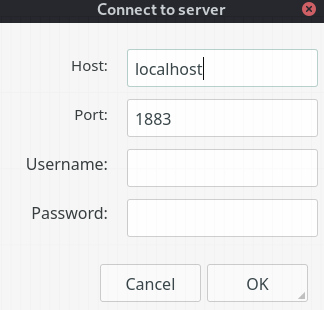
\includegraphics[width=0.5\textwidth]{img/app_connect.png}
            \caption{Okno nawiązywania połączenia}
            \label{fig:app_connect}
        \end{figure}
    
    
    \subsection{Panel parametrów}
        Dolna część okna podzielona jest na trzy części.
        
        \begin{itemize}
            \item Panel parametrów regulatora.
            \item Panel widoczności wykresów.
            \item Panel z aktualnymi danymi.
        \end{itemize}
        
        Pierwsza z nich udostępnia interfejs do dynamicznej zmiany nastaw regulatora 

    \subsection{Graf}
    Interfejs zawiera wszystkie elementy niezbędne do wygodnej obsługi urządzenia.
    
    \begin{figure}[ht]
        \centering
        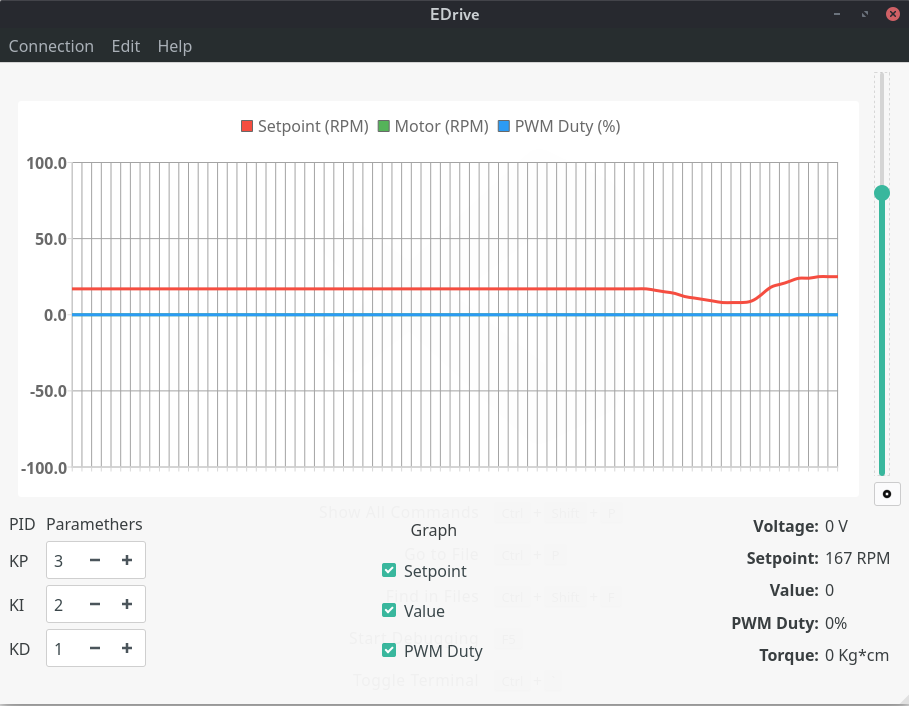
\includegraphics[width=1\textwidth]{img/app_ui.png}
        \caption{Interfejs użytkownika}
        \label{fig:app_ui}
    \end{figure} % APP - interfejs użytkownika
    
    
  \chapter{Podsumowane} % podsumowanie

    \addcontentsline{toc}{chapter}{\bibname}
    
    
  \begin{thebibliography}{9}

    \bibitem{qt}
        Qt Development Frameworks: Dokumentacja biblioteki Qt \newline
        \url{https://doc.qt.io/qt-5/} \newline
        Dostęp 14.09.2021
    
    \bibitem{mostek}
        STMicroelectronics: Dokumentacja L298H \newline
        \url{https://www.sparkfun.com/datasheets/Robotics/L298_H_Bridge.pdf} \newline
        Dostęp 14.09.2021
    
    \bibitem{esp32}
        Espressif Systems: Dokumentacja mikrokontrolera ESP32
        \url{https://www.espressif.com/sites/default/files/documentation/esp32_datasheet_en.pdf} \newline
        Dostęp 14.09.2021
    
    \bibitem{esp_module}
        Espressif Systems: Dokumentacja modułu ESP32­WROOM­32UE
        \url{https://www.espressif.com/sites/default/files/documentation/esp32_datasheet_en.pdf} \newline
        Dostęp 14.09.2021
    
    \bibitem{mqtt}
        OASIS: Dokumentacja standardu MQTT 5.0 \newline
        \url{https://docs.oasis-open.org/mqtt/mqtt/v5.0/mqtt-v5.0.pdf} \newline
        Dostęp 14.09.2021
    
    \bibitem{książka}
        V.P. Eloranta, J. Koskinen, M. Leppanen, V. Reijonen: 
        Designing Distributed Control Systems: A Pattern Language Approach, 
        Wiley, 2014.
    
    \bibitem{moore}
        Kenneth Flamm: Measuring Moore’s Law: Evidence from Price, Cost, and Quality Indexes  \newline
        \url{https://www.imf.org/-/media/Files/Conferences/2017-stats-forum/session-6-kenneth-flamm.ashx} \newline
        Dostęp 15.09.2021
    
    \bibitem{esp-idf}
        Espressif Systems: Dokumentacja ESP-IDF  \newline
        \url{https://docs.espressif.com/projects/esp-idf/en/latest/esp32/} \newline
        Dostęp 15.09.2021
    
    \bibitem{freertos}
        Amazon Web Services: Dokumentacja FreeRTOS  \newline
        \url{https://www.freertos.org/a00106.html} \newline
        Dostęp 15.09.2021
    
    \bibitem{szereg}
        Wikipedia: Szereg wartości  \newline
        \url{https://pl.wikipedia.org/wiki/Szereg_warto\%C5\%9Bci} \newline
        Dostęp 17.09.2021
    
    \bibitem{dzielnik}
        Wikipedia: Dzielnik rezystorowy  \newline
        \url{https://en.wikipedia.org/wiki/Voltage\_divider} \newline
        Dostęp 17.09.2021
        
    \bibitem{gray}
        Robert W. Doran: The Gray Code  \newline
        \url{http://www.jucs.org/jucs_13_11/the_gray_code/jucs_13_11_1573_1597_doran.pdf} \newline
        Dostęp 27.09.2021
        
    \bibitem{enkoder}
        Siemens: Enkodery inkrementalne  \newline
        \url{https://publikacje.siemens-info.com/pdf/56/Motion\%20Control\%20-\%20Uk\%C5\%82ad\%20pomiarowy.pdf} \newline
        Dostęp 17.09.2021
        
    \bibitem{espressif}
        Espressif Systems: Producent SoC \newline
        \url{https://www.espressif.com}
        Dostęp 19.10.2021
  
    \bibitem{pwm}
        Robert McDowall: Fundamentals of HVAC Control Systems 
        
    \bibitem{pwm_center}
        Texas Instruments: Symmetric PWM Outputs Generation with the TMS320C14 DSP \newline
        \url{https://www.ti.com/lit/an/spra278/spra278.pdf}
        Dostęp 20.10.2021
        
    \bibitem{context}
        FreeRTOS FAQ: Context Switch Times \newline
        \url{https://www.freertos.org/FAQMem.html#ContextSwitchTime}
        Dostęp 8.11.2021        
        
     \bibitem{round_robin}
        Lawrence Williams: Round Robin Scheduling Algorithm \newline
        \url{https://www.guru99.com/round-robin-scheduling-example.html}
        Dostęp 8.11.2021        

     \bibitem{mosquitto}
        Strona domowa projektu Mosquitto \newline
        \url{https://mosquitto.org/}
        Dostęp 22.11.2021
  
     \bibitem{docker}
        Strona domowa projektu Docker \newline
        \url{https://www.docker.com/}
        Dostęp 22.11.2021  
        
     \bibitem{hor}
        Bruno Siciliano, Oussama Khatib: Springer Handbook of Robotics
        
        
    \bibitem{qt_mqtt_fig}
        Schemat działania modułu Qt MQTT  \newline
        \url{https://doc.qt.io/QtMQTT/mqtt-overview.html} \newline
        Dostęp 29.09.2021        
         
    \bibitem{freertos_fig}
        Topologia procesora z użyciem FreeRTOS  \newline
        \url{https://www.freertos.org/2020/02/simple-multicore-core-to-core-communication-using-freertos-message-buffers.html} \newline
        Dostęp 29.09.2021     
        
     \bibitem{h_bridge_conn_fig}
        Schemat podłączenia mostka H  \newline
        \url{https://forbot.pl/forum/topic/16-teoria-mostek-h-h-bridge-kompendium-dla-robotyka} \newline
        Dostęp 29.09.2021         
        
     \bibitem{engine_fig}
        Schemat wykorzystanego silnika  \newline
        \url{https://www.dfrobot.com/product-1619.html} \newline
        Dostęp 29.09.2021
                
     \bibitem{h_bridge_fig}
        Schemat wykorzystanego mostka  \newline
        \url{https://www.sparkfun.com/datasheets/Robotics/L298_H_Bridge.pdf} \newline
        Dostęp 29.09.2021
        
     \bibitem{mqtt_schematic_fig}
        Schemat działania protokołu MQTT  \newline
        \url{https://en.wikipedia.org/wiki/MQTT} \newline
        Dostęp 29.09.2021
        
     \bibitem{qt_s&s_fig}
        System sygnałów i slotów \newline
        \url{https://doc.qt.io/qt-5/signalsandslots.html} \newline
        Dostęp 29.09.2021
        
     \bibitem{esp_fig}
        Wykorzystana jednostka centralna \newline
        \url{https://www.digikey.pl/product-detail/pl/espressif-systems/ESP32-WROOM-32U-16MB/1904-1028-1-ND/9381737} \newline
        Dostęp 29.09.2021
        
     \bibitem{pwm_fig}
        Przebiegi sygnału PWM \newline
        \url{https://developer.android.com/things/sdk/pio/pwm} \newline
        Dostęp 20.10.2021
        
    \bibitem{freertos_task_fig}
        Możliwe stany procesów w FreeRTOS \newline
        \url{https://microcontrollerslab.com/wp-content/uploads/2017/07/FreeRTOS-tasks-state.png} \newline
        Dostęp 8.11.2021

  \end{thebibliography}
  
   % bibliografia
    
    \listoffigures % spis rysunków
    \listoflistings % spis kodu
\end{document}